\documentclass[UTF8]{ctexart}
\usepackage{tikz,pgfplots}
\usetikzlibrary{arrows,intersections,angles,patterns}
\usepgflibrary{arrows.meta}
\pgfplotsset{compat=1.15}
\usepgfplotslibrary{fillbetween}
\usepgflibrary{decorations.markings}

\begin{document}
    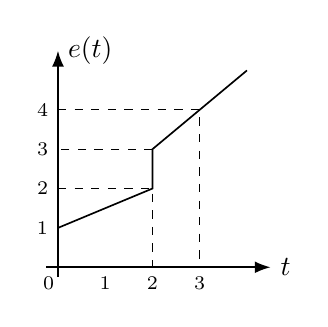
\begin{tikzpicture}[xscale=0.6,yscale=0.5]
            \draw [semithick][-{Latex}](-0.25,0) -- (4.5,0) node[right] {$t$};
            \draw [semithick][-{Latex}] (0,-0.25) -- (0,5.5) node[right] {$e(t)$} ;
            %坐标,标注
            \draw (-0.2,0) node[below] {\scriptsize $0$} (1,0) node[below] {\scriptsize $1$} ; 
            \draw [thin,dashed] (0,2) node[left] {\scriptsize $2$ }--(2,2)--(2,0) node[below] {\scriptsize $2$ };
            \draw [thin,dashed] (0,4) node[left] {\scriptsize $4$ }--(3,4)--(3,0) node[below] {\scriptsize $3$ };
            \draw [thin,dashed] (2,3)--(0,3) node[left] {\scriptsize $3$ };
            %矩形脉冲
            \draw [semithick] (0,1) node[left] {\scriptsize $1$ }-- (2,2) 
            --(2,3) --(4,5);   
    \end{tikzpicture}
    
    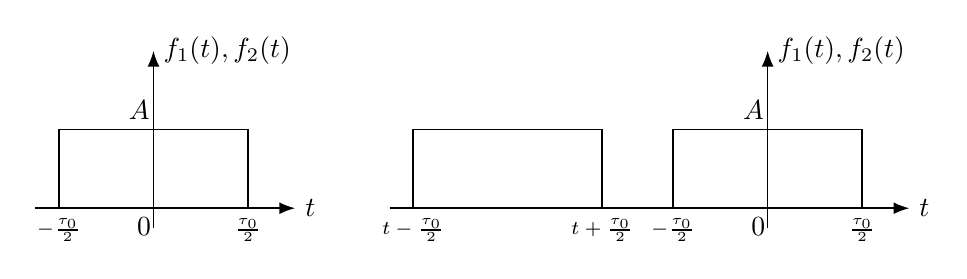
\begin{tikzpicture}[xscale=0.6,yscale=0.5]
        %坐标轴;
            \draw [semithick][-{Latex}](-2.5,0) -- (3,0) node[right] {$t$};
            \draw [semithick][-{Latex}] (0,-0.5) -- (0,4) node[right] {$f_1(t),f_2(t)$} ;
        %坐标,标注
            \draw (-0.2,0) node[below] {$0$} (-0.3,2) node[above] {$A$} ; 
            %\draw [thin,dashed] (0,2)--(2,2);
        %矩形脉冲
            \draw [semithick] (-2,0 )node[below] {\scriptsize $-\frac {\tau_0} 2$}-- (-2,2) -- (2,2)--(2,0) node[below] {\scriptsize $\frac {\tau_0} 2$};
            \begin{scope}[xshift=13cm, yshift=0cm]
                \draw [semithick][-{Latex}](-8,0) -- (3,0) node[right] {$t$};
                \draw [semithick][-{Latex}] (0,-0.5) -- (0,4) node[right] {$f_1(t),f_2(t)$} ;
        %坐标,标注
                \draw (-0.2,0) node[below] {$0$} (-0.3,2) node[above] {$A$} ; 
                %\draw [thin,dashed] (0,2)--(2,2);
        %矩形脉冲
                \draw [semithick] (-2,0 )node[below] {\scriptsize $-\frac {\tau_0} 2$}-- (-2,2) -- (2,2)--(2,0) node[below] {\scriptsize $\frac {\tau_0} 2$};
                \draw [semithick] (-7.5,0 )node[below] {\scriptsize $t-\frac {\tau_0} 2$}-- (-7.5,2) -- (-3.5,2)--(-3.5,0) node[below] {\scriptsize $t+\frac {\tau_0} 2$};
            \end{scope}
    \end{tikzpicture}

    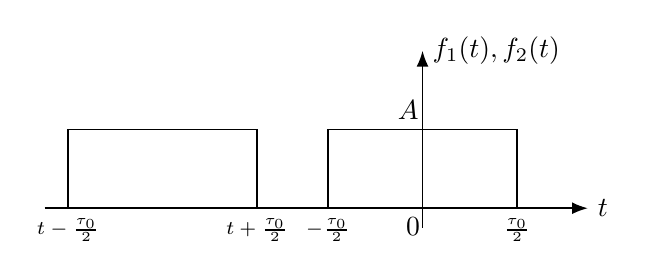
\begin{tikzpicture}[xscale=0.6,yscale=0.5]
        %坐标轴;
            \draw [semithick][-{Latex}](-8,0) -- (3.5,0) node[right] {$t$};
            \draw [semithick][-{Latex}] (0,-0.5) -- (0,4) node[right] {$f_1(t),f_2(t)$} ;
        %坐标,标注
            \draw (-0.2,0) node[below] {$0$} (-0.3,2) node[above] {$A$} ; 
            %\draw [thin,dashed] (0,2)--(2,2);
        %矩形脉冲
            \draw [semithick] (-2,0 )node[below] {\scriptsize $-\frac {\tau_0} 2$}-- (-2,2) -- (2,2)--(2,0) node[below] {\scriptsize $\frac {\tau_0} 2$};
            \draw [semithick] (-7.5,0 )node[below] {\scriptsize $t-\frac {\tau_0} 2$}-- (-7.5,2) -- (-3.5,2)--(-3.5,0) node[below] {\scriptsize $t+\frac {\tau_0} 2$};
    \end{tikzpicture}

    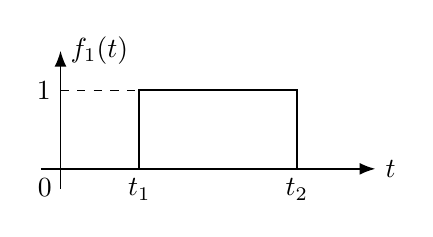
\begin{tikzpicture}[scale=1]
        %坐标轴;
        \draw [semithick][-{Latex}] (-0.25,0) -- (4,0) node[right] {$t$};
        \draw [semithick][-{Latex}] (0,-0.25) -- (0,1.5) node[right] {$f_1(t)$} ;
        %坐标
        \draw (-0.2,0) node[below] {0} (0,1) node[left] {1} ; 
        \draw [thin,dashed] (0,1)--(1,1);
        %矩形脉冲
        \draw [semithick](1,0 )node[below] {$t_1$}-- (1,1) -- (3,1)--(3,0) node[below] {$t_2$};
    \end{tikzpicture}

    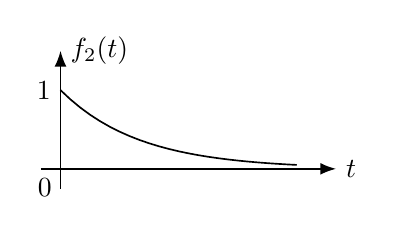
\begin{tikzpicture}[scale=1]
        %坐标轴;
        \draw [semithick][-{Latex}] (-0.25,0) -- (3.5,0) node[right] {$t$};
        \draw [semithick][-{Latex}] (0,-0.25) -- (0,1.5) node[right] {$f_2(t)$} ;
        %坐标
        \draw (-0.2,0) node[below] {0} (0,1) node[left] {1} ; 
        %指数曲线
        \draw [semithick,domain=0:3] plot (\x,{exp(-\x)}); %(\x,{sin(\x r)});
    \end{tikzpicture}

    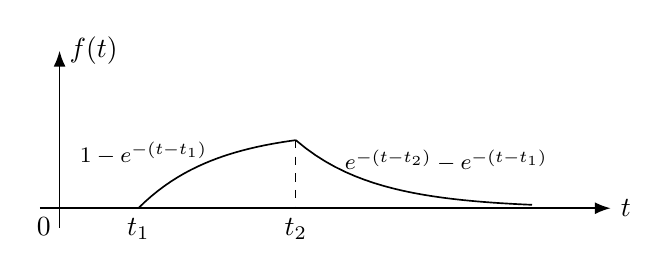
\begin{tikzpicture}[scale=1]
        %坐标轴;
        \draw [semithick][-{Latex}] (-0.25,0) -- (7,0) node[right] {$t$};
        \draw [semithick][-{Latex}] (0,-0.25) -- (0,2) node[right] {$f(t)$} ;
        %坐标
        \draw (-0.2,0) node[below] {0} (1,0) node[below] {$t_1$} (3,0) node[below] {$t_2$}
        (2,0.7) node[left] {\footnotesize $1-e^{-(t-t_1)}$} (3.5,0.6) node[right] {\footnotesize $e^{-(t-t_2)}-e^{-(t-t_1)}$};
        \draw [thin,dashed] (3,0.865)--(3,0); 
        %指数曲线
        \draw [semithick,domain=1:3] plot (\x,{1-exp(-(\x-1))});
        \draw [semithick,domain=3:6] plot (\x,{exp(-(\x-3))-exp(-(\x-1))});
    \end{tikzpicture}

    
    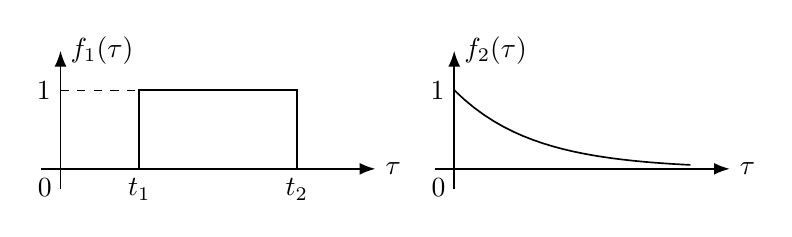
\begin{tikzpicture}[scale=1]
        %坐标轴;
        \draw [semithick][-{Latex}] (-0.25,0) -- (4,0) node[right] {$\tau$};
        \draw [semithick][-{Latex}] (0,-0.25) -- (0,1.5) node[right] {$f_1(\tau)$} ;
        %坐标
        \draw (-0.2,0) node[below] {0} (0,1) node[left] {1} ; 
        \draw [thin,dashed] (0,1)--(1,1);
        %矩形脉冲
        \draw [semithick](1,0 )node[below] {$t_1$}-- (1,1) -- (3,1)--(3,0) node[below] {$t_2$};
    

        \begin{scope}[scale=1,xshift=5cm, yshift=0cm]
            %坐标轴;
            \draw [semithick][-{Latex}] (-0.25,0) -- (3.5,0) node[right] {$\tau$};
            \draw [semithick][-{Latex}] (0,-0.25) -- (0,1.5) node[right] {$f_2(\tau)$} ;
            %坐标
            \draw (-0.2,0) node[below] {0} (0,1) node[left] {1} ; 
            %指数曲线
            \draw [semithick,domain=0:3] plot (\x,{exp(-\x)}); %(\x,{sin(\x r)});
        \end{scope}
    \end{tikzpicture}

    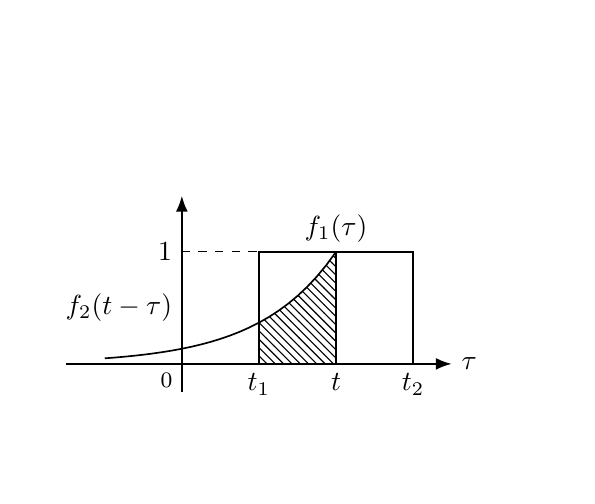
\begin{tikzpicture}[scale=1]
        \begin{axis}[hide axis,xmin=-2, xmax=5,ymin=-1, ymax=3]
       		%坐标轴;
        	\draw [semithick][-{Latex}] (-1.5,0) -- (3.5,0) node[right] {$\tau$};
        	\draw [semithick][-{Latex}] (0,-0.25) -- (0,1.5);
        	%坐标
        	\draw (-0.2,0) node[below] {\footnotesize 0} (0,1) node[left] {1} ; 
			\draw [thin,dashed] (0,1)--(1,1);
			\draw [semithick] (2,1)--(2,0) node[below] {$t$}; 
			\coordinate [label=left:$f_2(t-\tau)$] (A) at (0,0.5);
			\coordinate [label=above:$f_1(\tau)$] (B) at (2,1);
			%矩形脉冲
        	\draw [semithick] (1,0) node[below] {$t_1$}-- (1,1) -- (3,1)--(3,0) node[below] {$t_2$};
        	%指数曲线
       		\draw [semithick,name path=A,domain=-1:2] plot (\x,{exp(\x-2)});
            \path[name path=B]
            (\pgfkeysvalueof{/pgfplots/xmin},0) --
            (\pgfkeysvalueof{/pgfplots/xmax},0);
            \addplot[pattern=north west lines] fill between[of=A and B,
            soft clip={domain=1:2},
            ];
        \end{axis}
    \end{tikzpicture}

    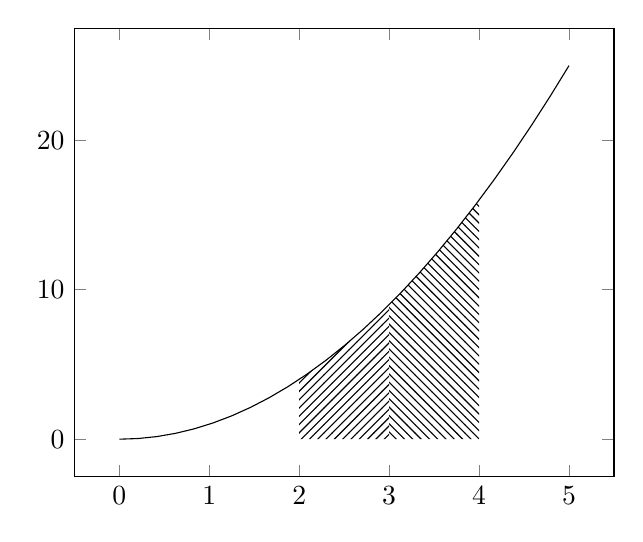
\begin{tikzpicture}
        \begin{axis}
            \addplot[name path=A,domain=0:5] {x^2};
            \path[name path=B]
            (\pgfkeysvalueof{/pgfplots/xmin},0) --
            (\pgfkeysvalueof{/pgfplots/xmax},0);
            \addplot[pattern=north west lines] fill between[of=A and B,
            soft clip={domain=3:4},
            ];
            \addplot[pattern=north east lines] fill between[of=A and B,
            soft clip={domain=2:3},
            ];
        \end{axis}
    \end{tikzpicture}

    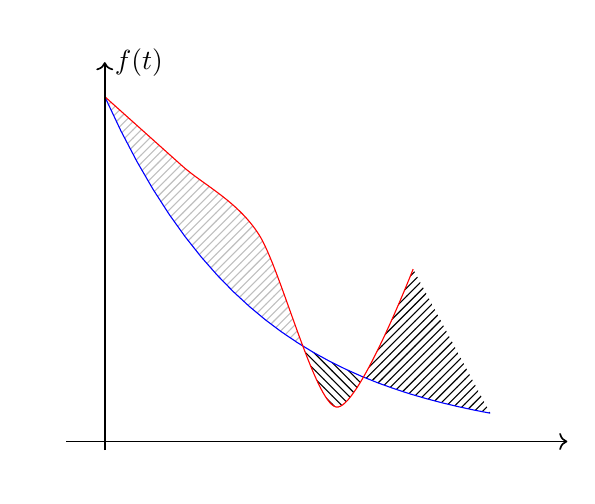
\begin{tikzpicture}
        \begin{axis}[hide axis,xmin=-1, xmax=6,ymin=-1, ymax=12]
            %\draw [blue,name path=A,domain=0:5] plot (\x,{10*exp(-0.5*\x)}); %(\x,{sin(\x r)});
            \addplot[blue,name path=A,domain=0:5] {10*exp(-0.5*x)};%{x^2};
            \addplot[red,name path=B,smooth] table {
            x y
            0 10
            1 8
            2 6
            3 1
            4 5
            };
           \addplot fill between[of=A and B,
           split,
           every segment no 0/.style={pattern color=gray!50,pattern=north east lines},
           every segment no 1/.style={pattern=north west lines},
           every segment no 2/.style={pattern=north east lines}];
            \draw [semithick][->] (0,-0.25) -- (0,11) node[right] {$f(t)$} ;
            \draw [semithick][->] (-0.5,0) -- (6,0) node[right] {$t$};
        \end{axis}
         
        % \draw [semithick][->] (0.5,-0.25) -- (0.5,8) node[right] {$f(t)$} ;
    \end{tikzpicture}

    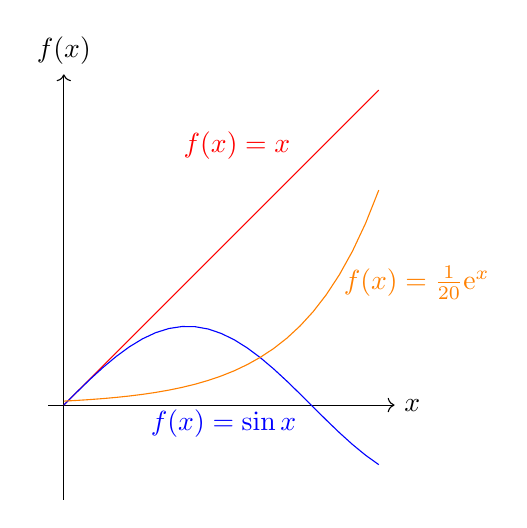
\begin{tikzpicture}[domain=0:4,label/.style={postaction={
            decorate,
            decoration={
            markings,
            mark=at position .75 with \node #1;}}}]
        %\draw[very thin,color=gray] (-0.1,-1.1) grid (3.9,3.9);
        \draw[->] (-0.2,0) -- (4.2,0) node[right] {$x$};
        \draw[->] (0,-1.2) -- (0,4.2) node[above] {$f(x)$};
        \draw[red,label={[above left]{$f(x)=x$}}] plot (\x,\x);
        \draw[blue,label={[below left]{$f(x)=\sin x$}}] plot (\x,{sin(\x r)});
        \draw[orange,label={[right]{$f(x)= \frac{1}{20} \mathrm e^x$}}] plot (\x,{0.05*exp(\x)});
    \end{tikzpicture}

    
\end{document}